%  Beamer slide example.

\documentclass[9pt]{beamer}
% \setbeameroption{show only notes}
%\setbeameroption{show notes}

\usepackage[utf8]{inputenc}
\usetheme{inria}
\usepackage{helvet}
\usepackage{graphicx}

\author{Maurice Bremond \and Gaëtan Harter}

\title[Intégration continue]{L'Intégration Continue}
% \subtitle{Dans un contexte de développement Inria}
\subtitle{Présentation IJD}

% Automatically insert a "new section" page at each section.
\AtBeginSection[]{
  \begin{frame}[plain]
    \partpage
  \end{frame}
}
% \inriaswitchcolors COLOR
%
% Where COLOR is one of red, blue, orange, darkblue, violet,
% pastelgreen, grey, or green.
\newcommand{\inriaswitchcolors}[1]{%
  \pgfaliasimage{figfootline}{figfootline-#1}% !!!
  \pgfaliasimage{figbackground}{figbackground-#1}% !!!
  \pgfaliasimage{figbackground}{figbackground-#1}% !!!
}

% frame with toc for current subsection
\newcommand{\tocsubsection}[1]{
  \begin{frame}
    \tableofcontents[
      currentsubsection,
      sectionstyle=show/shaded,
      subsectionstyle=show/shaded,
      subsubsectionstyle=show/show/shaded
    ]
    #1
  \end{frame}
}
% starting the document
% *********************
\begin{document}
% titlepage
% ---------
\begin{frame}[plain]
  \titlepage
\end{frame}
% table of contents
% -----------------
\begin{frame}{\textcolor{inriaGrey}{Table des matières}}
  \tableofcontents
\end{frame}



% Introduction
% ************

\inriaswitchcolors{red}
\section{Quid de l'intégration continue}

\subsection{Qu'est-ce que c'est}
\begin{frame}{\subsecname}

  Contenu

\end{frame}



% L'intégration continue à Inria
% ******************************
\inriaswitchcolors{blue}
\section{L'intégration continue à Inria}




% Retour d'expérience
% *******************
\inriaswitchcolors{green}
\section{Un retour d'expérience}
\frame{\tableofcontents[currentsection]
  \note{Vous avez besoin d'intégration continue\\}
  \note{Exemple mon expérience personnelle}
}

\subsection{Contexte de développement}
\tocsubsection{\note{Justifié de le faire pour moi, vous reconnaître sur certains points}}

\subsubsection{FIT Equipex - Future Internet of Things}
\begin{frame}{\subsubsecname} %{\subsecname}
  \note[item]{Equipex: 'equipement excellence' projet FR}
  \note[item]{Future Internet of Thing.}
  \note[item]{plusieurs plateformes}
  \note[item]{Durée de 10 ans}
  \note[item]{}
  \note[item]{IOT-LAB - description slide suivant}

  \begin{center}
    \begin{tabular}{ l l }
      
\includegraphics[width=0.2\textwidth]{images/logo_invest_avenir} &
      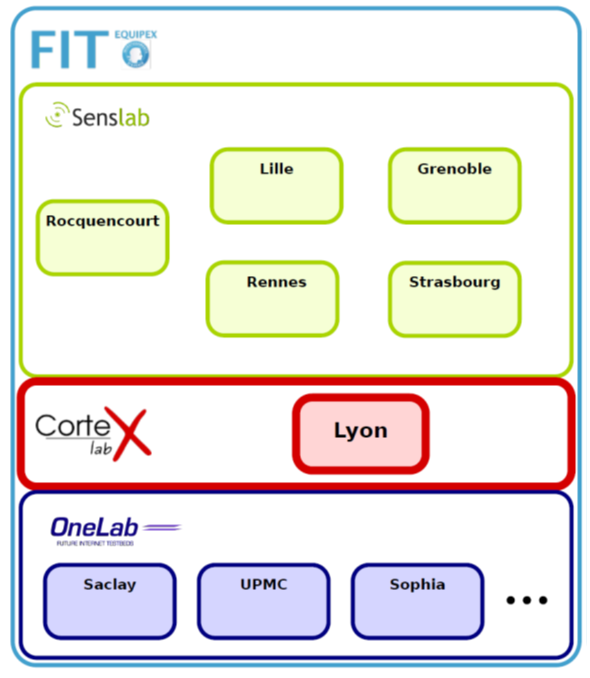
\includegraphics[width=0.5\textwidth]{images/fit_equipex} \\
    \end{tabular}
  \end{center}
\end{frame}


\subsubsection{Plateforme de réseau de capteurs: FIT IoT-LAB}
\begin{frame}{\subsubsecname} %{\subsecname}
  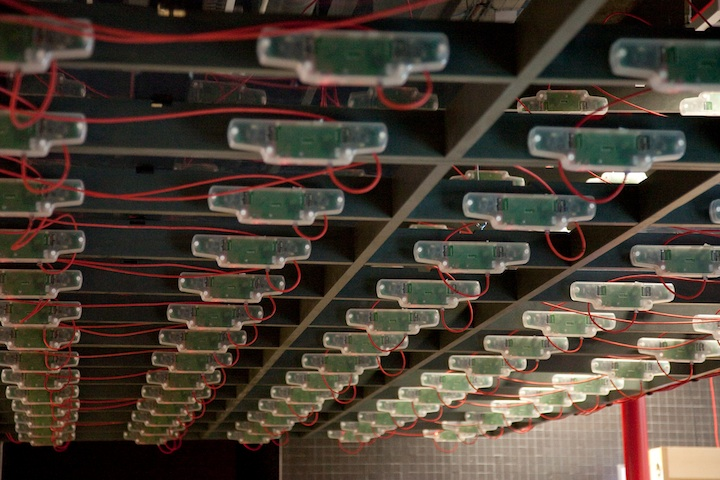
\includegraphics[width=\textwidth]{images/senslab_nodes}
  \note[item]{IoT-LAB: réseaux de capteurs 'objets connectés', 3000}
  \note[item]{Objets qui communiquent courte distance, et joignable depuis l'internet}
  \note[item]{Mis à disposition des chercheurs}
  \note[item]{2 générations de capteurs}
\end{frame}

\begin{frame}{\subsubsecname} %{\subsecname}
  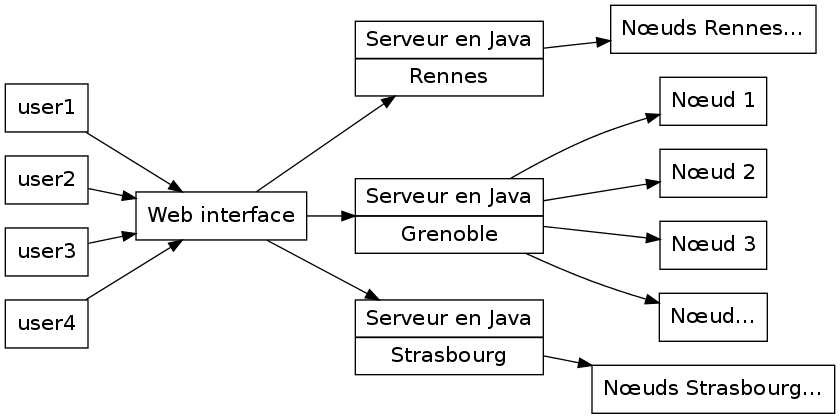
\includegraphics[width=\textwidth]{images/fit_architecture}
  \note{Exemple d'un chercheur voulant expérimenter sur les réseaux de capteurs}
  \note[item]{Se connecter sur l'interface web}
  \note[item]{Réserver un grand nombre de nœuds capteurs (3k dispos)}
  \note[item]{Déployer des programmes dessus}
  \note[item]{Interragir avec eux par connection série}
  \note[item]{Monitorer leur fonctionnement, conso, radio}
\end{frame}


\subsubsection{Un nœud capteur IoT-LAB}
\begin{frame}{\subsubsecname} %{\subsecname}
  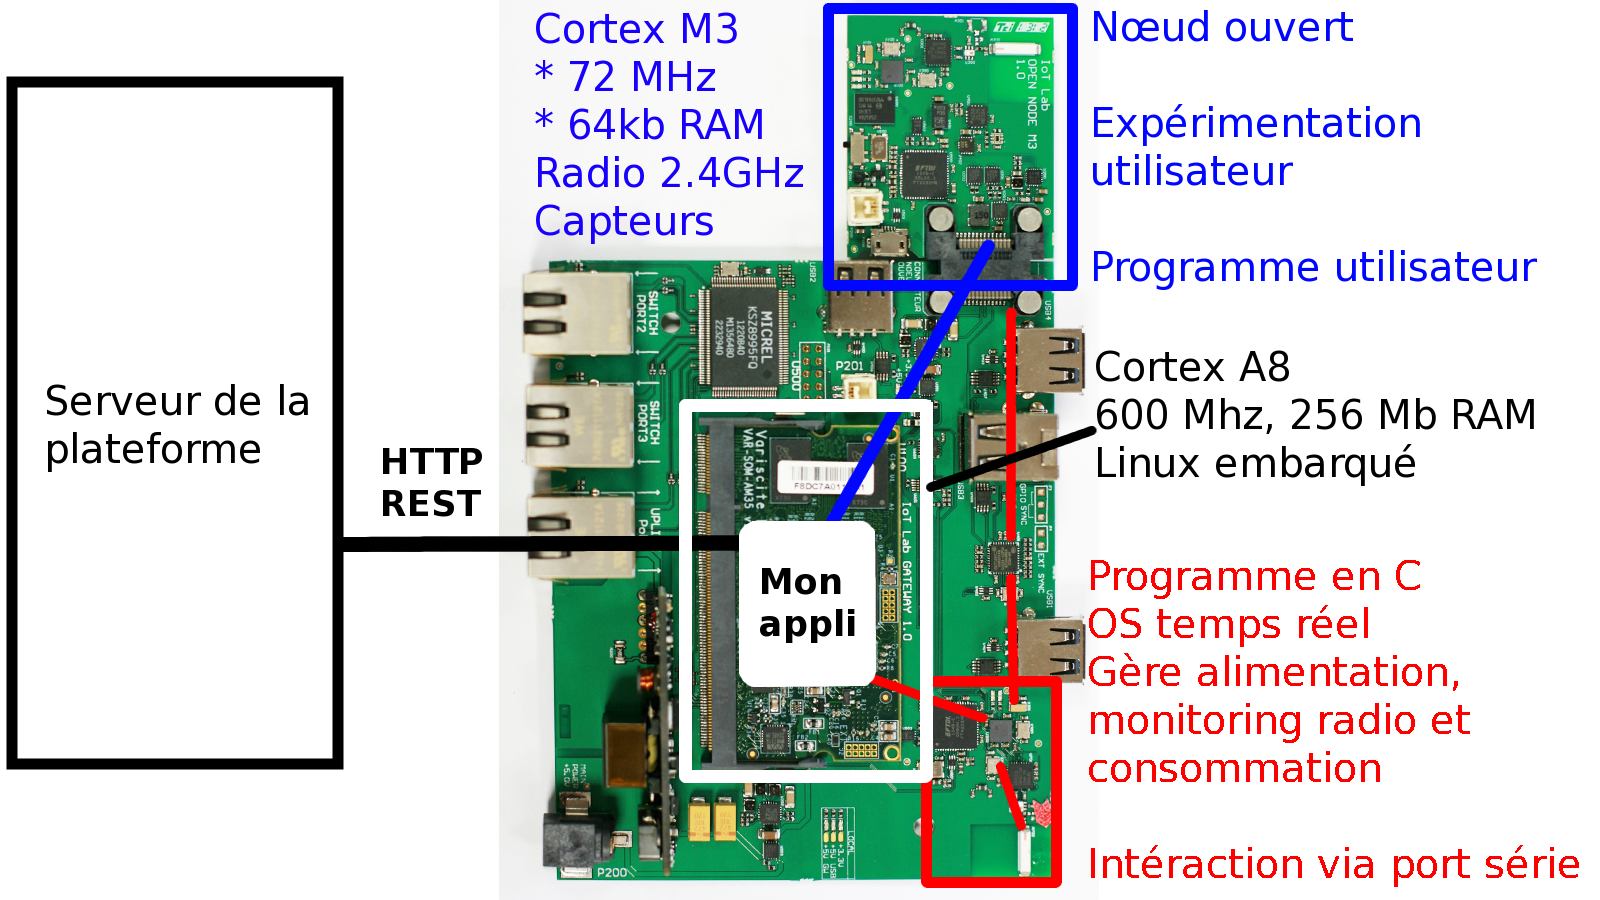
\includegraphics[width=\textwidth]{images/gateway_m3_annote}
\end{frame}

\subsubsection{Contexte de l'application}
\begin{frame}{\subsubsecname} %{\subsecname}
  \begin{itemize}
    \item Python + C (+ outils compilés externes)
    \item Application mise en production (QoS)
    \item Exécution sur une carte ARM avec Linux embarqué (perf...)
    \item Intéractions extérieures
    \item multithread, multiprocess
  \end{itemize}
\end{frame}


\subsubsection{Pourquoi avoir mis place de l'intégration continue}
\begin{frame}{\subsubsecname} %{\subsecname}
  \begin{itemize}
    \item Sources d'erreurs non déterministes
      \note[item]{Dépendance à du matériel}
      \note[item]{Dépendance à des programmes qui ne sont pas sur la même machine}
      \note[item]{Multithread et multiprocess}
      \note[item]{}
    \item Logiciel final doit être fiable
      \note[item]{service 24/7}
      \note[item]{Coût d'un bug: Debug, mise à jour}
      \note[item]{Large échelle, proba d'apparition d'un bug}
      \note[item]{}
    \item J'avais envie d'essayer
    \item La chose qui m'a décidée…
  \end{itemize}
\end{frame}

\subsubsection{J'avais besoin d'un seul test}
\begin{frame}[fragile]{\subsubsecname} %{\subsecname}
  \setbeamercovered{transparent}

  \begin{verbatim}

  def thread_redirection(self):
      while not self.stop:
          self.proc = subprocess.Popen(['socat', ...)
          self.proc.wait()
          if 0 != self.proc.returncode:
              # Gestion de l'erreur

  def stop(self):
      while self.is_alive():
          self.proc.terminate()
          time.sleep(0.1)

  \end{verbatim}

  \onslide <2-> Test sur carte: '\texttt{ImportError: No module named arpgarse}'


\end{frame}



\subsection{Outils mis en place}
\tocsubsection{
  \note[item]{Juste une overview, un exemple}
  \note[item]{Quelques possibilité et contraintes}
  \note[item]{En utilisant ci.inria.fr}
}

\subsubsection{Présentation des outils}
\begin{frame}{Outils mis en place}

  Gestionnaire de versions: \texttt{git} \\ ~ \\

  \begin{tabular}{ l | l l | p{3.5cm} }
    Language         & \texttt{Python}     & \texttt{C}    & Exploitation dans Jenkins \\ \hline
    Script de build  & \texttt{setuptools} & \texttt{Make} & Bash~shell, \texttt{EnvInject} \texttt{virtualenv}\\
    Compilation      & ~                   & \texttt{gcc}  & ~ \\
    Tests            & \texttt{nose}, \texttt{unittest}, \texttt{mock}
                     & \texttt{gtest} \texttt{(C++)}
                     & Junit, Chuck Norris\\
    Couverture       & \texttt{nose-xcover}
                     & \texttt{gcov}, \texttt{gcovr}
                     & Cobertura \\
   Qualité de code  & \texttt{pylint}, \texttt{pep8} & ~  & Violations \\
    ~ & ~  & ~ & \\
    Lignes de code   &  $3000$        &  $1500$  &  $0$  \\
    Lignes de tests  &  $1600 + 400$  &  $1300$  &  $0$  \\
% 1600 tests U + 400 tests intégration
    Lignes de build  &  $300$         &  $170$   &  $50$ \\

    \note[item]{Gestion de version, partagée avec d'autres projets}
    \note[item]{Correspondance entre outils mis en place et Jenkins, \textbf{fichiers générés}}
    \note[item]{Types d'outils les uns après les autres}
    \note[item]{Pylint remplace compilation python}
    \note[item]{}
    \note[item]{1600 tests U + 400 tests intégration}
    \note[item]{SQLite 3.8 == 1084 * plus de tests que de code 84k source (hors blank et commentaires)}
  \end{tabular}
\end{frame}


\subsubsection{Jenkins}
\begin{frame}{Présentation outils}{Jenkins}
  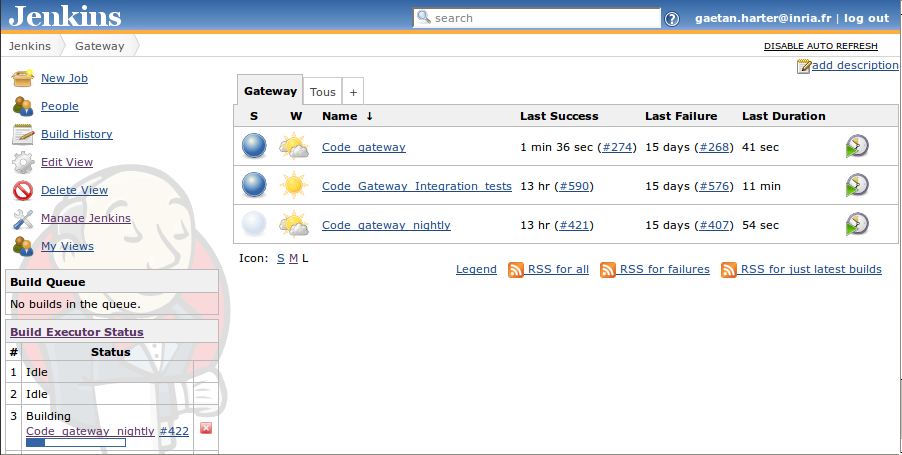
\includegraphics[width=\linewidth]{images/jenkins}
  \note[item]{2 types}
  \note[item]{Sur carte cible \textbf{Thales}}
  \note[item]{Lancement des tests, à la main et toute les nuits}
\end{frame}

\begin{frame}{Configuration d'un build}{Jenkins}
  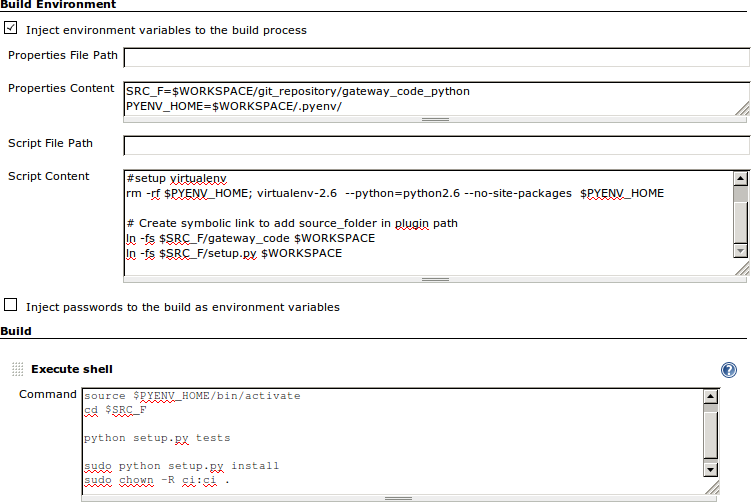
\includegraphics[width=\linewidth]{images/build_configuration}
\end{frame}


\begin{frame}{Cobertura}{Jenkins}
        % Pour moi, l'outil le plus important (après Chuck Norris forcément)
  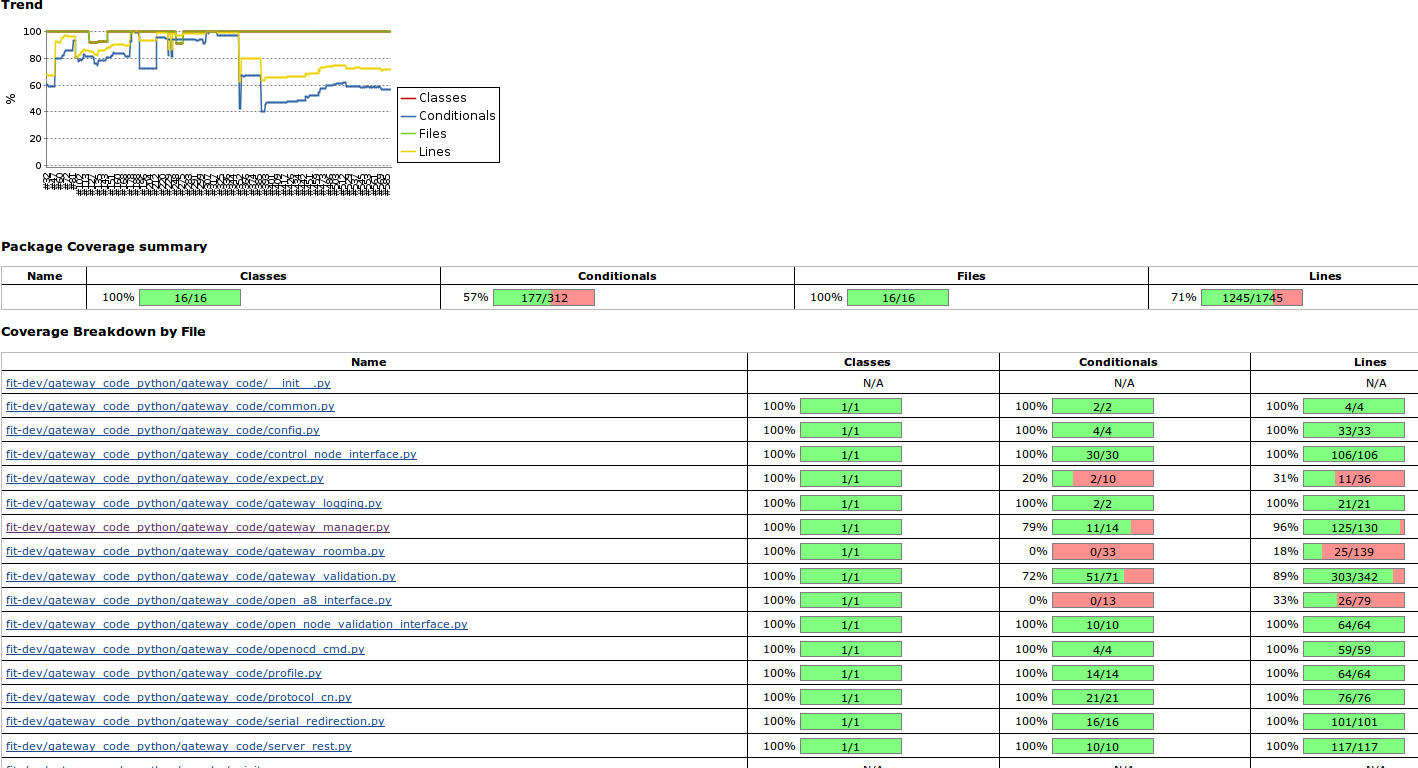
\includegraphics[width=\linewidth]{images/cobertura}\\
\end{frame}
\begin{frame}{Junit - Violations}{Jenkins}
  \begin{center}
        % Juste pour montrer
    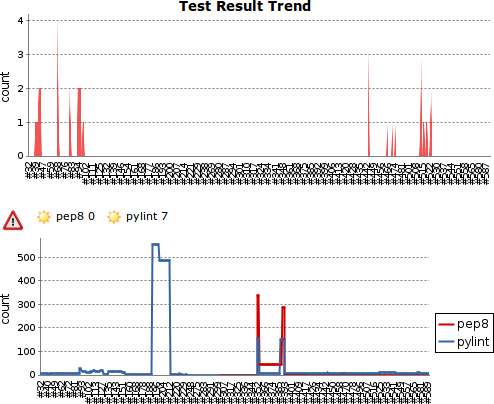
\includegraphics[height=0.8\textheight]{images/junit_violations}\\
  \end{center}
\end{frame}
\begin{frame}{Chuck Norris}{Jenkins}
  % Le plus important des plugins
  \begin{center}
    \begin{tabular}{ l |l }
      Build KO & Build OK \\ \hline
        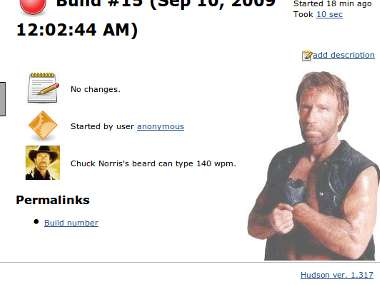
\includegraphics[height=4cm]{images/chuck_full} &
      
\includegraphics[height=4cm]{images/chuck_happy}
        %
\includegraphics[height=4cm]{images/chuck_angry}
      \\
    \end{tabular}
  \end{center}
  Chuck Norris Facts:
  \begin{itemize}
    \item Chuck Norris can unit test an entire application with a single assert.
    \item Chuck Norris can divide by zero.
    \item ...
  \end{itemize}
\end{frame}




\subsection{Bilan}
\tocsubsection


\subsubsection{Développement logiciel}
\begin{frame}{\subsubsecname}{\subsecname}
  \note{GROS SLIDE}

  \begin{itemize}
    \item Mise en place d'un script de \texttt{build}
      \note[item]{Procédure de test, même 1 seul test}
      \note[item]{Procédure simple dans un script}
      \note[item]{}
    \item Tests nombreux et lancés en continu
      \note[item]{Gestion des cas d'erreurs}
      \note[item]{Détection de problèmes tot (perf réimplèm en C}
      \note[item]{simplification de l'implem}
      \note[item]{dev itératif}
      \note[item]{Detection d'erreurs rares}
      \note[item]{}
    \item Couverture de code
      \note[item]{Même si $<100\%$, savoir ce qui est 'validé' et ce qui ne l'est pas}
    \item Qualité de code
      \note[item]{Python: Remplace la phase de compilation (vérification syntaxique)}
      \note[item]{Détection statique d'erreurs}
      \note[item]{Standardisation de la mise en forme, lisibilité (PEP8)}
      \note[item]{}
  \end{itemize}
  Maîtrise et confiance dans le logiciel développé
\end{frame}

\subsubsection{Personnel}
\begin{frame}{\subsubsecname}{\subsecname}
  \begin{itemize}
    \item Découverte de beaucoup d'outils
    \item Maîtrise des languages et leur écosystème
    \item Confort dans le développement
    \item Retours positifs après premières utilisations
    \item J'aimerai maintenant pouvoir l'appliquer à d'autres choses
  \end{itemize}
  \note[item]{Rassurant}
  \note[item]{Je peux tester!}
\end{frame}

\subsubsection{Voies d'amélioration}
\begin{frame}{\subsubsecname}{\subsecname}
  \begin{itemize}
    \item Passer les configurations Jenkins dans des scripts versionnés
    \item Grouper Python et C dans le build python
    \item Inclusion d'autres développeurs
    \item 100\% de couverture de code
  \end{itemize}
\end{frame}


\begin{frame}{The End}
  Merci d'avoir écouté.
\end{frame}


\end{document}
